\documentclass[11pt, hyperref={urlcolor=red,% Liens vers une page web
            linkcolor=blue, %Liens internes au document
            colorlinks=true}]{beamer}  
            
\usetheme{Warsaw} 

%thèmes prédéfinis de Beamer 
%Antibes, boxes, classic, Darmstadt, Madrid
% Montpellier, Warsaw, Bergen, Berkeley, Goettingen, sidebar


%%%%%%%Tit\title{Titre principal}

\title[suites]{Exemples du cours Variables aléatoires 2019/2020}
%\subtitle{Sous titre}
\author[F.Junier]{Fr\'ed\'eric Junier}
\institute[Le Parc]{{\centering Lyc\'ee du Parc \\
1 Boulevard Anatole France \\ 69006 Lyon }}
\date[\today]{\today}

\usepackage{etex}

%%%%%%%%%%%%Encodage du fichier source %%%%%%%%%%%
\usepackage[T1]{fontenc}
\usepackage[utf8]{inputenc}

\usepackage{lmodern}
\usepackage{url}
\usepackage[np]{numprint}


%%%%%%%%%%%%Là encore il y a de grosses différences entre le monde anglo-saxon et les francophones.Le séparateur des décimales est un point en anglais et une virgule en français. Leséparateur des milliers est une virgule en anglais et une espace insécable en français. Ilest préférable d’utiliser le package numprint (\usepackage{numprint}) qui associé àfrenchb produira la bonne typographie.
%123456789 = 123456789 \numprint{123456789} = 123 456 789  \numprint{3,1415926535897932384626} = 3,141 592 653 589 793 238 462 6  \numprint{12.34} = 12,34  En plus tu peux préciser les unités de cette façon : \numprint[kg]{12.34} = 12,34 kg ou encore \numprint[\degres C]{22} = 22°C Si tu veux utiliser le raccourci \np{} au lieu de \numprint{}, il te faut charger le package de cette façon : \usepackage[np]{numprint}


%%%%%%%%%%PSTricks%%%%%%%%%%%%

\usepackage{pstricks,pst-plot,pst-text,pst-tree,pst-eps,pst-fill,pst-node,pst-math,pstricks-add,pst-xkey,pst-eucl}


%%%%%%%Tikz%%%%%%%%%%%%%%%
\usepackage{pgf,tikz,tkz-tab}
% Pour les tableaux de signes ou de variations avec tkz-tab voir https://zestedesavoir.com/tutoriels/439/des-tableaux-de-variations-et-de-signes-avec-latex/#1-13389_tikz-un-package-qui-en-a-dans-le-ventre
\usetikzlibrary{arrows}
\usetikzlibrary{shapes.geometric}
\usetikzlibrary{shapes.geometric}
\usetikzlibrary{petri}
\usetikzlibrary{decorations}
\usetikzlibrary{arrows}
\usetikzlibrary{math}
 %Variables must be declared in a tikzmath environment but
       % can be used outside
%       \tikzmath{int \n; \n = 508; \x1 = 1; \y1 =1; 
%                   %computations are also possible
%                    \x2 = \x1 + 1; \y2 =\y1 +3; } 


%%%%%%%%%%%%%%%%%%%%%%%%%%%%%%%%%%%%%%%%
%%%%%%%%%%%Commandes Tikz Perso%%%%%%%%%%%%%%%

% Définition des nouvelles options xmin, xmax, ymin, ymax
% Valeurs par défaut : -3, 3, -3, 3
\tikzset{
xmin/.store in=\xmin, xmin/.default=-3, xmin=-3,
xmax/.store in=\xmax, xmax/.default=3, xmax=3,
ymin/.store in=\ymin, ymin/.default=-3, ymin=-3,
ymax/.store in=\ymax, ymax/.default=3, ymax=3,
}
% Commande qui trace la grille entre (xmin,ymin) et (xmax,ymax)
\newcommand {\grille}[2]
{\draw[help lines,black, thick] (\xmin,\ymin) grid[xstep=#1, ystep=#2] (\xmax,\ymax);}
% Commande \axes
\newcommand {\axes} {
\draw[->,very thick] (\xmin,0) -- (\xmax,0);
\draw[->,very thick] (0,\ymin) -- (0,\ymax);
\draw (0.95*\xmax, 0) node[above] {$x$};
\draw (0, 0.95*\ymax) node[left] {$y$};
}
% Commande qui limite l?affichage à (xmin,ymin) et (xmax,ymax)
\newcommand {\fenetre}
{\clip (\xmin,\ymin) rectangle (\xmax,\ymax);}

%Exemple d'utilisation

%\begin{center}
%\begin{tikzpicture} [xmin=-2,xmax=2,ymin=0,ymax=5]
%\grille{1} \axes \fenetre
%\draw plot[smooth] (\x,\x^2);
%\end{tikzpicture}
%\end{center}

%style pour la perspective cavalière française
%voir Tikz pour l'impatient page 68
\tikzset{math3d/.style=
{x= {(-0.353cm,-0.353cm)}, z={(0cm,1cm)},y={(1cm,0cm)}}}

%%%%%%%Symbole pour code calculatrice%%%%%%

%Flèche remplie pour défilement de menu

\newcommand{\flechefillright}{
\begin{tikzpicture}[scale=0.15] \fill (0,0)--(2,1)--(0,2)--cycle;
\end{tikzpicture}}

%%%%%%%%%%%%%Symboles pour calculatrice Casio%%%%
\newcommand{\execasio}{\Pisymbol{psy}{191}} %Retour chariot
\newcommand{\dispcasio}{\begin{pspicture}(.1,.1)\pspolygon*(.1,0)(.1,.1)\end{pspicture}} %Triangle « Disp »
\newcommand{\dispcasiotikz}{\begin{tikzpicture}[scale=0.2]
\fill (0,0) -- (1,0) -- (1,1) -- cycle;
\end{tikzpicture}} %Triangle « Disp »
%


%%%%%%%%%%%%%%%%%%%Présentation de codes sources%%%%%%%%%%%%%%%%%
\usepackage{listings}
%On utilise l?environnement lstlisting pour insérer
%un code source.
%En plus de l?environnement lstlisting, on peut également utiliser la
%commande \lstinline qui fonctionne comme la commande \verb, en ce
%sens qu?on peut utiliser n?importe quel caractère comme délimiteur. Enfin,
%la commande \lstinputlisting permet de charger un code source depuis
%un fichier externe.
%Il y a deux manières de préciser des options : soit via l?option de l?envi-
%ronnement ou de la commande, soit en utilisant la commande \lstset
%qui permet de définir des options de manière globale.

\lstset{ %
  language=Python,                % the language of the code
  basicstyle=\ttfamily,           % the size of the fonts that are used for the code
  %numbers=left,                   % where to put the line-numbers
  numberstyle=\tiny,  % the style that is used for the line-numbers
  %stepnumber=2,                   % the step between two line-numbers. If it's 1, each line 
                                  % will be numbered
  %numbersep=5pt,                  % how far the line-numbers are from the code
  backgroundcolor=\color{white},      % choose the background color. You must add \usepackage{color}
  showspaces=false,               % show spaces adding particular underscores
  showstringspaces=false,         % underline spaces within strings
  showtabs=false,                 % show tabs within strings adding particular underscores
  frame=single,                   % adds a frame around the code
  rulecolor=\color{black},        % if not set, the frame-color may be changed on line-breaks within not-black text (e.g. comments (green here))
  tabsize=4,                      % sets default tabsize to 2 spaces
  captionpos=b,                   % sets the caption-position to bottom
  breaklines=true,                % sets automatic line breaking
  breakatwhitespace=false,        % sets if automatic breaks should only happen at whitespace
  %title=\lstname,                   % show the filename of files included with \lstinputlisting;
                                  % also try caption instead of title
  breakindent=1cm,
  keywordstyle=\color{blue},          % keyword style
  commentstyle=\color{red},       % comment style
  %stringstyle=\ttfamily\color{green},         % string literal style
  escapeinside={\%*}{*)},            % if you want to add LaTeX within your code
  morekeywords={*,...},              % if you want to add more keywords to the set
  deletekeywords={...}              % if you want to delete keywords from the given language
  upquote=true,columns=flexible,
xleftmargin=1cm,xrightmargin=1cm,
 inputencoding=utf8,			%Les lignes qui suivent sont pour le codage utf8
  extendedchars=true,
  literate=%
            {é}{{\'{e}}}1
            {è}{{\`{e}}}1
            {ê}{{\^{e}}}1
            {ë}{{\¨{e}}}1
            {û}{{\^{u}}}1
            {ù}{{\`{u}}}1
            {â}{{\^{a}}}1
            {à}{{\`{a} }}1
            {î}{{\^{i}}}1
            {ô}{{\^{o}}}1
            {ç}{{\c{c}}}1
            {Ç}{{\c{C}}}1
            {É}{{\'{E}}}1
            {Ê}{{\^{E}}}1
            {À}{{\`{A}}}1
            {Â}{{\^{A}}}1
            {Î}{{\^{I}}}1
}

\lstdefinestyle{rond}{
  numbers=none,
  frameround =tttt
}

\lstdefinestyle{compil}{
  numbers=none,
  backgroundcolor=\color{gristclair}
}
%\lstset{language=Python,basicstyle=\small , frame=single,tabsize=4,showspaces=false,showtabs=false,showstringspaces=false,numbers=left,numberstyle=\tiny , extendedchars=true}

%%%%%%%%%%%AmsMaths%%%%%%
\usepackage{amsmath,amsfonts,amssymb}
\usepackage{pifont,fourier}
\usepackage{ bclogo}


%%%%%Commande \DeclareMathOperator pour définir de nouveaux opérateurs (en lettres romaines droites)%%%%%
%\DeclareMathOperator{\sh}{sh}
%\DeclareMathOperator{\ch}{ch}

%%%%%%%%%%%%%%%%%%Maths divers%%%%%%%%%%%%%%%%%%%%%%%%%
%Delimiteurs
\newcommand{\delim}[3]{\raise #1\hbox{$\left #2\vbox to #3{}\right.$}}


%%%%%%%%%%%%%Nombres%%%%%%%%%%%%%%%%

%Ensemble prive de...
%\newcommand{\prive}{\boi}%{\backslash}

%Ensembles de nombres%%%%%%%%%%%%%%%%%
\newcommand{\R}{\mathbb{R}}
\newcommand{\N}{\mathbb{N}}
\newcommand{\D}{\mathbb{D}}
\newcommand{\Z}{\mathbb{Z}}
\newcommand{\Q}{\mathbb{Q}}
\newcommand{\C}{\mathbb{C}}
\newcommand{\df}{~\ensuremath{]0;+\infty[}~}
\newcommand{\K}{\mathbb{K}}

%%%%%%%%Arithmetique%%%%%%%%%%
%PGCD, PPCM
\newcommand{\PGCD}{\mathop{\rm PGCD}\nolimits}
\newcommand{\PPCM}{\mathop{\rm PPCM}\nolimits}

%Intervalles
\newcommand{\interoo}[2]{]#1\, ;\, #2[}
\newcommand{\Interoo}[2]{\left]#1\, ;\, #2\right[}
\newcommand{\interof}[2]{]#1\, ;\, #2]}
\newcommand{\Interof}[2]{\left]#1\, ;\, #2\right]}
\newcommand{\interfo}[2]{[#1\, ;\, #2[}
\newcommand{\Interfo}[2]{\left[#1\, ;\, #2\right[}
\newcommand{\interff}[2]{[#1\, ;\, #2]}
\newcommand{\Interff}[2]{\left[#1\, ;\, #2\right]}
%\newcommand\interentiers #1#2{[\! [#1\, ;\, #2]\! ]}
\newcommand{\interentiers}[2]{\llbracket #1\, ;\, #2\rrbracket}
%


%%%%%%%%%%%%%%Nombres complexes%%%%%

\newcommand{\ic}{\text{i}}
%\newcommand{\I}{\text{i}}
\newcommand{\im}[1]{\text{Im}\left(#1\right)}
\newcommand{\re}[1]{\text{Re}\left(#1\right)}
\newcommand{\Arg}[1]{\text{arg}\left(#1\right)}
\newcommand{\Mod}[1]{\left[#1\right]}
%Parties entière, réelle, imaginaire, nombre i
\newcommand{\ent}[1]{\text{E}\left(#1\right)}
\renewcommand{\Re}{\mathop{\rm Re}\nolimits}
\renewcommand{\Im}{\mathop{\rm Im}\nolimits}
\renewcommand{\i}{\textrm{i}}

%%%%%%%%%%%Probabilites et statistiques%%%%%
\newcommand{\loibinom}[2]{\mathcal{B}\left(#1\ ; \ #2 \right)}
\newcommand{\loinorm}[2]{\mathcal{N}\left(#1\ ; \ #2 \right)}
\newcommand{\loiexp}[1]{\mathcal{E}\left(#1\right)}
\newcommand{\proba}[1]{\mathbb{P}\big(#1\big)}
\newcommand{\probacond}[2]{\mathbb{P}_{#2}\big(#1\big)}
\newcommand{\esperance}[1]{\mathbb{E}\left(#1\right)}
\newcommand{\variance}[1]{\mathbb{V}\left(#1\right)}
\newcommand{\ecart}[1]{\sigma\left(#1\right)}
\newcommand{\dnormx}{\frac{1}{\sqrt{2\pi}} \text{e}^{-\frac{x^2}{2}}}
\newcommand{\dnormt}{\frac{1}{\sqrt{2\pi}} \text{e}^{-\frac{t^2}{2}}}
\newcommand{\nbalea}[2]{\reinitrand[first=#1, last=#2, counter=num]  \rand $\thenum$}  %retourne un entier aleatoire antre les bornes #1 et #2 comprises
%Covariance
\newcommand{\cov}{\mathop{\rm cov}\nolimits}
%


%%%%%%%%%%Analyse%%%%%%%%%%%

%%%%%%%%%%%Courbe%%%%%%%%%%%%
\newcommand{\courbe}[1]{\ensuremath{\mathcal{C}_{#1}}}

%%%%%%%Fonction exponentielle%%%%%
\newcommand{\fe}{~fonction exponentielle~}
\newcommand{\e}{\text{e}}

%Fonction cotangente
\newcommand{\cotan}{\mathop{\rm cotan}\nolimits}
%%%%%%%%%%%%%%%%%%%%%%%%%%%%%%%%%%%%%%%%%
%
%Fonctions hyperboliques
\newcommand{\ch}{\mathop{\rm ch}\nolimits}
\newcommand{\sh}{\mathop{\rm sh}\nolimits}


%%%%%%%%%%%%%%Limites%%%%%%
\newcommand{\limite}[2]{\lim\limits
_{x \to #1} #2}
\newcommand{\limitesuite}[1]{\lim\limits
_{n \to +\infty} #1}
\newcommand{\limiteg}[2]{\lim\limits
_{\substack{x \to #1 \\ x < #1 }} #2}
\newcommand{\limited}[2]{\lim\limits
_{\substack{x \to #1 \\ x > #1 }} #2}

%%%%%%%%%%Continuité%%%%%%%%%%%
\newcommand{\TVI}{théorème des valeurs intermédiaires}

%%%%%%%%%%%Suites%%%%%%%%%%%%
\newcommand{\suite}[1]{\ensuremath{\left(#1_{n}\right)}}
\newcommand{\Suite}[2]{\ensuremath{\left(#1\right)_{#2}}}
%

%%%%%%%%%%%%%%%Calcul intégral%%%%%%
\newcommand{\dx}{\ensuremath{\text{d}x}}		% dx
\newcommand{\dt}{\ensuremath{\text{d}t}}		% dt
\newcommand{\dtheta}{\ensuremath{\text{d}\theta}}		% dtheta
\newcommand{\dy}{\ensuremath{\text{d}y}}		% dy
\newcommand{\dq}{\ensuremath{\text{d}q}}		% dq

%%%Intégrale%%%
\newcommand{\integralex}[3]{\int_{#1}^{#2} #3 \ \dx}
\newcommand{\integralet}[3]{\int_{#1}^{#2} #3 \ \dt}
\newcommand{\integraletheta}[3]{\int_{#1}^{#2} #3 \ \dtheta}

%%%%%Equivalent%%
\newcommand{\equivalent}[1]{\build\sim_{#1}^{}}

%o et O%%%%
\renewcommand{\o}[2]{\build o_{#1\to #2}^{}}
\renewcommand{\O}[2]{\build O_{#1\to #2}^{}}



%%%%%%%%%%%%%%%Geometrie%%%%%%%%%%%%%%%%%%%%%%%

%%%%%%%%%%%%%%%Reperes%%%%%%%%%%%%%%
\def\Oij{\ensuremath{\left(\text{O},~\vect{\imath},~\vect{\jmath}\right)}}
\def\Oijk{\ensuremath{\left(\text{O},~\vect{\imath},~ \vect{\jmath},~ \vect{k}\right)}}
\def\Ouv{\ensuremath{\left(\text{O},~\vect{u},~\vect{v}\right)}}
\renewcommand{\ij}{(\vec\imath\, ;\vec\jmath\,)}
\newcommand{\ijk}{(\vec\imath\, ;\vec\jmath\, ;\vec k\,)}
\newcommand{\OIJ}{(O\,;\, I\,;\, J\,)}
\newcommand{\repere}[3]{\big(#1\, ;\,\vect{#2} ;\vect{#3}\big)}
\newcommand{\reperesp}[4]{\big(#1\, ;\,\vect{#2} ;\vect{#3} ;\vect{#4}\big)}

%%%%%%%%%Coordonnees%%%%%%%%%%%%%%
\newcommand{\coord}[2]{(#1\, ;\, #2)}
\newcommand{\bigcoord}[2]{\big(#1\, ;\, #2\big)}
\newcommand{\Coord}[2]{\left(#1\, ;\, #2\right)}
\newcommand{\coordesp}[3]{(#1\, ;\, #2\, ;\, #3)}
\newcommand{\bigcoordesp}[3]{\big(#1\, ;\, #2\, ;\, #3\big)}
\newcommand{\Coordesp}[3]{\left(#1\, ;\, #2\, ;\, #3\right)}
\newcommand{\Vcoord}[3]{\begin{pmatrix} #1 \\ #2 \\ #3 \end{pmatrix}}
%Symboles entre droites
%\newcommand{\paral}{\sslash}
\newcommand{\paral}{\mathop{/\!\! /}}
%

%%%%%%%%%Produit scalaire, Angles%%%%%%%%%%
\newcommand{\scal}[2]{\vect{#1} \, \cdot \, \vect{#2}}
\newcommand{\Angle}[2]{\left(\vect{#1} \, , \, \vect{#2}\right)}
\newcommand{\Anglegeo}[2]{\left(\widehat{\vect{#1} \, ; \, \vect{#2}}\right)}
\renewcommand{\angle}[1]{\widehat{#1}}
\newcommand{\anglevec}[2]{\left(\vect {#1}\, ,\,\vect {#2} \right)}
\newcommand{\anglevecteur}[2]{(#1\, , \, #2)}
\newcommand{\Anglevec}[2]{(\vecteur{#1}\, ,\,\vecteur{#2})}
\newcommand{\prodscal}[2]{#1 \, \cdot \, #2}
%


%Arc
%\newcommand{\arc}[1]{\wideparen{#1}}
\newcommand{\arcoriente}[1]{\overset{\curvearrowright}{#1}}
%
%


%%%%%%%%%%%%%%%Normes%%%%%%%%%%%%%%%%
\newcommand{\norme}[1]{\left\| #1\right\|}
\newcommand{\normebis}[1]{\delim{2pt}{\|}{9pt}\! #1\delim{2pt}{\|}{9pt}}
\newcommand{\normetriple}[1]{\left |\kern -.07em\left\| #1\right |\kern -.07em\right\|}
\newcommand{\valabs}[1]{\big| \, #1 \, \big|}
%

%%%%%%%%%%%%%%%%%%%%%%%%%%%Degré%%%%%%
%\newcommand{\Degre}{\ensuremath{^\circ}}
%La commande \degre est déjà définie dans le package babel

%%%%%%%%%%Vecteurs%%%%%%%%%%%
\newcommand{\vect}[1]{\mathchoice%
{\overrightarrow{\displaystyle\mathstrut#1\,\,}}%
{\overrightarrow{\textstyle\mathstrut#1\,\,}}%
{\overrightarrow{\scriptstyle\mathstrut#1\,\,}}%
{\overrightarrow{\scriptscriptstyle\mathstrut#1\,\,}}}



%%%%%%%%%%%%%Algebre%%%%%%%%%%%%%%%


%%%%%%%%%%Systemes%%%%%%%%%%%
%Systemes
\newcommand{\sys}[2]{
\left\lbrace
 \begin{array}{l}
  \negthickspace\negthickspace #1\\
  \negthickspace\negthickspace #2\\
 \end{array}
\right.\negthickspace\negthickspace}
\newcommand{\Sys}[3]{
\left\lbrace
 \begin{array}{l}
  #1\\
  #2\\
  #3\\
 \end{array}
\right.}
\newcommand{\Sysq}[4]{
\left\lbrace
 \begin{array}{l}
  #1\\
  #2\\
  #3\\
  #4\\
 \end{array}
\right.}
%
%

%%%%%%%%%%%%%%%%Matrices%%%%%%%%%%%%%%%%%%
%Comatrice
\newcommand{\com}{\mathop{\rm com}\nolimits}
%
%
%Trace
\newcommand{\tr}{\mathop{\rm tr}\nolimits}
%
%
%Transposee
\newcommand{\transposee}[1]{{\vphantom{#1}}^t\negmedspace #1}
%
%
%Noyau
\newcommand{\Ker}{\mathop{\rm Ker}\nolimits}
%
%

%
%Matrices
\newcommand{\Mn}{\mathcal M_n}
\newcommand{\matrice}[4]{
\left(
 \begin{array}{cc}
  #1 & #2 \\
  #3 & #4
 \end{array}
\right)}

\newcommand{\Matrice}[9]{
\left(
 \begin{array}{ccc}
  #1 & #2 & #3\\
  #4 & #5 & #6\\
  #7 & #8 & #9
 \end{array}
\right)}
\newcommand{\Vect}[3]{
\left(\negmedspace
 \begin{array}{c}
  #1\\
  #2\\
  #3
 \end{array}\negmedspace
\right)}
\newcommand{\Ideux}{\matrice{1}{0}{0}{1}}
\newcommand{\Itrois}{\Matrice{1}{0}{0}{0}{1}{0}{0}{0}{1}}
%
%
%Determinants
\newcommand{\determinant}[4]{
\left|
 \begin{array}{cc}
  #1 & #2 \\
  #3 & #4
 \end{array}
\right|}
\newcommand{\Determinant}[9]{
\left|
 \begin{array}{ccc}
  #1 & #2 & #3\\
  #4 & #5 & #6\\
  #7 & #8 & #9
 \end{array}
\right|}

%%%%%%%%%%%%%%Calculs en Latex%%%%%%%%%%%%%

\usepackage[first=1,last=100]{lcg}  %%%%%%%générer des nombres pseudo aléatoires
%%%%
\usepackage{calc} %   pour faire des calculs%%


%%%%Mise en page%%%%%
\usepackage{fancybox}
\usepackage{lastpage}
\usepackage{hyperref}
%À mettre dans le préambule pour faire apparaitre le plan à chaque section 

\AtBeginSection[ ]
{
\begin{frame}<beamer>
\frametitle{Plan}
\tableofcontents[currentsection]
\end{frame}
}

%%%%%%%¨Puces%%%%%%%%%%%%
\usepackage{enumerate}


%%%%%%%%%%%%Graphiques%%%%%%%%%%%%%%
\usepackage{graphicx,pgf}				
\usepackage{pstricks,pst-plot,pst-text,pst-tree,pst-eps,pst-node,pst-math,pstricks-add}
 


%%%%%%Numérotation des automatismes%%%%%%
\newcounter{autocompteur}
\setcounter{autocompteur}{0}
\newcommand{\automatisme}[1]{\addtocounter{autocompteur}{1}\frametitle{Automatisme  \theautocompteur  \textit{ thème : #1}}}
%%%%%%%%%%%%%%%%%%%%%%%%%%%%%%%%%%%%%%%%%%%%%%%%

%%%%%%%%%%%%%%%Francisation%%%%%%%%%%%%%%
\usepackage[french]{babel}
\frenchbsetup{StandardLists=true}

%%%%%%%%%%%%%%%%%%%%%%%%%%%%%%%%%%%%%%%%%



\begin{document}

\frame{\titlepage}

 


\begin{frame}
\frametitle{Table des matières}
\begin{itemize}
    \item \hyperlink{activite2}{Activité 2}
    \item \hyperlink{capacite1}{Capacité 1}
    \item \hyperlink{capacite2}{Capacité 2}
    \item \hyperlink{capacite3}{Capacité 3}
    \item \hyperlink{capacite4}{Capacité 4}
     \item \hyperlink{algo1}{Algorithmique 1}
     \item \hyperlink{capacite5}{Capacité 5}
    \item \hyperlink{capacite6}{Capacité 6}
    \item \hyperlink{algo2}{Algorithmique 2}
     \item \hyperlink{algo3}{Algorithmique 3}
       \item \hyperlink{algo4}{Algorithmique 4}
        \item \hyperlink{algo5}{Algorithmique 5}
\end{itemize}

\end{frame}



\begin{frame}
\frametitle{Activité 2,  partie 1}
\label{activite2}

On lance trois fois de suite une pièce équilibrée et l'on note après chaque lancer si le côté sorti est  pile (noté $P$) ou  face (noté $F$) .

\begin{itemize}
\pause \item Représentation  à l'aide d'un arbre de l'ensemble des issues possibles de cette expérience aléatoire. Toutes les branches ont une probabilité de $\frac{1}{2}$

\begin{center}
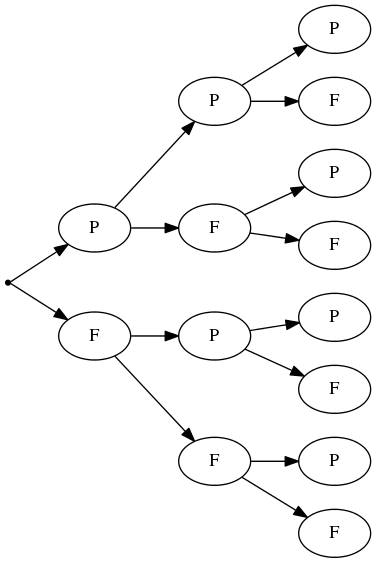
\includegraphics[scale=0.2]{images/pieces-3lancers.png}
\end{center}

\end{itemize}  


\end{frame}



\begin{frame}
\frametitle{Activité 2, partie 2}


On lance trois fois de suite une pièce équilibrée et l'on note après chaque lancer si le côté sorti est  pile (noté $P$) ou  face (noté $F$) .

\begin{itemize}
\pause \item L'univers $\Omega$ de cette expérience aléatoire compte $2^{3}=8$ issues équiprobables.
\pause \item Soit l'événement A = \og{} Obtenir exactement un Pile \fg{}. Cet événement est réalisé par $3$ issues donc $\proba{A}=\frac{3}{8}$.
\pause \item Soit l'événement B = \og{} Obtenir au moins un Pile \fg{}. Cet événement a pour contraire $\overline{B}$ = \og{} N'obtenir aucun Pile \fg{} dont la probabilité est  $\proba{\overline{B}}=\frac{1}{8}$. On en déduit que $\proba{B}=\frac{7}{8}$.

\end{itemize}  


\end{frame}


\begin{frame}
\frametitle{Activité 2 : déterminer une ligne de niveau, partie 3}


On définit à partir de  cette expérience aléatoire un jeu qui consiste  à gagner $1$ €  pour chaque face sorti  et à perdre $1,1$ € pour chaque pile sorti.

La fonction  $G$ de $\Omega$ dans $\R$ associe à une issue de l'expérience aléatoire  le gain du joueur.

\begin{itemize}
\pause \item La variable aléatoire $G$ prend quatre valeurs distinctes : $1+1+1=3$, $1+1-1,1=0,9$, $1-1,1-1,1=-1,2$ et $-1,1-1,1-1,1=-3,3$.
\pause \item Loi de la variable aléatoire $G$ :
  \begin{itemize}
\pause \item  $\mathbb{P}(G = 3)= \frac{1}{8}$ et  $\mathbb{P}(G = 0,9)= \frac{3}{8}$
 \pause \item  $\mathbb{P}(G = -1,2)= \frac{3}{8}$ et  $\mathbb{P}(G = -3,3)= \frac{1}{8}$
\end{itemize}  
\end{itemize} 

\end{frame}



\begin{frame}
\frametitle{Capacité 1,  partie 1}
\label{capacite1}
On lance deux fois de suite un dé tétraédrique  équilibré dont les quatre faces sont numérotées $1$, $2$, $3$ et $4$.
Lors de chaque lancer, on note le nombre porté par la face du dessous  et on fait la somme des deux nombres obtenus successivement.

La probabilité d'obtenir une somme paire est-elle égale à $\frac{1}{2}$ ?

\begin{itemize}
\pause \item L'univers de cette expérience aléatoire est constitué de $4^{2}=16$ issues équiprobables de la forme (face dé 1, face dé 2). 


\pause \item L'événement A = \og{} la somme est paire \fg{} est constitué de $2 \times 2 = 4$ couples de faces paires et $2 \times 2=4$  couples de faces impaires. La probabilité de A est donc $\proba{A}=\frac{8}{16}=\frac{1}{2}$.

\end{itemize}



\end{frame}


\begin{frame}
\frametitle{Capacité 1,  partie 2}
On lance deux fois de suite un dé   équilibré  à $n$ faces dont les  faces sont numérotées $1$, $2$, \ldots  $n$.
Lors de chaque lancer, on note le nombre porté par la face du dessous  et on fait la somme des deux nombres obtenus successivement.

\begin{itemize}
\pause \item L'univers de cette expérience aléatoire est constitué de $n^{2}$ issues équiprobables de la forme (face dé 1, face dé 2). 


\end{itemize}



\end{frame}





\begin{frame}
\frametitle{Capacité 1,  partie 3}
On lance deux fois de suite un dé   équilibré  à $n$ faces dont les  faces sont numérotées $1$, $2$, \ldots  $n$.
Lors de chaque lancer, on note le nombre porté par la face du dessous  et on fait la somme des deux nombres obtenus successivement.
Soit  l'événement A = \og{} La somme est paire  \fg{}. Une somme est paire si et seulement si les deux faces sont paires.

On distingue deux cas :


\begin{itemize}
\pause \item \underline{Premier cas : $n$ est pair :}  On a $n/2$ entiers pairs  et $n/2$ entiers impairs donc A est réalisé par $2 \times (n/2)^{2}=n^{2}/2$ issues et sa probabilité est  $\proba{A}=\frac{n^2/2}{n^2}=\frac{1}{2}$.


\pause \item \underline{Second cas :  $n$ est impair :}  On a $(n-1)/2$ entiers pairs  et $(n+1)/2$ entiers impairs donc A est réalisé par $((n-1)/2)^{2}+((n+1)/2)^{2}=(n^{2}+1)/2$ issues. La probabilité de $A$ est  donc $\proba{A}=\frac{(n^{2}+1)/2}{n^2}>\frac{1}{2}$.
\end{itemize}



\end{frame}

 

\begin{frame}
\label{capacite2}
\frametitle{Capacité 2,  partie 1}

On considère de nouveau  l'expérience aléatoire constituée de deux lancers successifs d'un dé tétraédrique équilibré et on note $X$ la variable aléatoire qui prend pour valeur la somme des nombres portés par les faces du dessous lors de chaque lancer.

La loi de probabilité de $X$ est donc :

\begin{center}
\begin{tabular}{|c|c|c|c|c|c|c|c|}
\hline 
k & 2 & 3 & 4 & 5 & 6  & 7 & 8\\ 
\hline 
$\proba{X=k}$ & 1/16 & 2/16 & 3/16  & 4/16   &  3/16 &  2/16 &  1/16  \\ 
\hline 
\end{tabular} 
\end{center}

\end{frame}




\begin{frame}
\frametitle{Capacité 2,  partie 2}
\begin{itemize}
\item $\proba{X=3} = 3/16$
	\pause \item $\proba{X\leqslant 3}=  \proba{X=2} + \proba{X=3}=1/16 + 2/16=3/16$
	\pause \item $\proba{X > 3}=1 - \proba{X\leqslant 2}=1-3/16=13/16$
	\pause \item $\proba{X \geqslant 3}=\proba{X > 3}+\proba{X=3}=13/16+2/16=15/16$.
\end{itemize}
	

\end{frame}



\begin{frame}
\frametitle{Capacité 3,  partie 1}


Une urne contient une boule rouge notée $R$, deux boules vertes notées $V_{1}$ et $V_{2}$ et deux boules bleues notées $B_{1}$ et $B_{2}$. On tire au hasard une boule dans l'urne. Si on tire la boule rouge on gagne $20$ euros, si on tire une boule verte on gagne $2$ euros et si on tire une boule bleue on perd $15$ euros.

On note $X$ le gain algébrique du joueur.

\begin{itemize}
	\pause \item Loi de probabilité de la variable aléatoire $X$ :
	
\begin{center}
\begin{tabular}{|c|c|c|c|}
\hline 
k & 20 & 2 & $-15$ \\ 
\hline 
$\proba{X=k}$ & $\frac{1}{5}$ & $\frac{2}{5}$ & $\frac{2}{5}$ \\ 
\hline 
\end{tabular} 
\end{center}

	\pause \item  $\proba{X \geqslant 0}=\proba{X=20}+\proba{X=2}=\frac{3}{5}$
	
	\pause \item On peut conjecturer que le gain moyen sur un grand nombre de parties va tendre presque sûrement vers $20 \times \proba{X=20} + 2 \times \proba{X=2}-15\times \proba{X=-15}=\frac{24}{5}-\frac{30}{5}=-\frac{6}{5}$.
	
\end{itemize}
	

\end{frame}



\begin{frame}
\frametitle{Capacité 3,  partie 2}


Une urne contient une boule rouge notée $R$, deux boules vertes notées $V_{1}$ et $V_{2}$ et deux boules bleues notées $B_{1}$ et $B_{2}$. On tire au hasard une boule dans l'urne. Si on tire la boule rouge on gagne $20$ euros, si on tire une boule verte on gagne $2$ euros et si on tire une boule bleue on perd $15$ euros.

On note $X$ le gain algébrique du joueur.

\begin{itemize}
	\pause \item Loi de probabilité de la variable aléatoire $X$ :
	
\begin{center}
\begin{tabular}{|c|c|c|c|}
\hline 
k & 20 & 2 & $-15$ \\ 
\hline 
$\proba{X=k}$ & $\frac{1}{5}$ & $\frac{2}{5}$ & $\frac{2}{5}$ \\ 
\hline 
\end{tabular} 
\end{center}

	
	\pause \item On peut conjecturer que le gain moyen sur un grand nombre de parties va tendre presque sûrement vers $20 \times \proba{X=20} + 2 \times \proba{X=2}-15\times \proba{X=-15}=\frac{24}{5}-\frac{30}{5}=-\frac{6}{5}$ et donc que sur un grand nombre de parties le gain moyen d'un joueur est presque sûrement négatif.
	
\end{itemize}
	

\end{frame}



\begin{frame}[fragile]
\label{algo1}
\frametitle{Algorithmique 1,  partie 1}

 Compléter la fonction \texttt{Python} ci-dessous pour que \texttt{somme\_n\_des(ndes, nfaces)} retourne la somme des résultats obtenus lors de \texttt{ndes} lancers d'un dé équilibré à \texttt{nfaces}.
 
\begin{itemize}

\pause \item 


\begin{lstlisting}[style=rond]
from random import randint

def somme_n_des(ndes, nfaces):
    s = 0
    for k in range(nfaces):
        s = s + randint(1, ndes)
    return s
\end{lstlisting}

\end{itemize}


\end{frame}




\begin{frame}[fragile]

\frametitle{Algorithmique 1,  partie 2}
Compléter la fonction \texttt{Python} ci-dessous pour que \texttt{gain\_urne()} retourne le gain algébrique du jeu décrit dans la capacité 3. 

 
\begin{itemize}

\pause \item 


\begin{lstlisting}[style=rond]
from random import random

def gain_urne():
    tirage = random()
    if tirage < 0.2:
        return 20
    elif tirage < 0.6:
        return 2
    else:
        return -15
\end{lstlisting}

\end{itemize}


\end{frame}





\begin{frame}[fragile]

\frametitle{Algorithmique 1,  partie 3}
Un élève a complété la fonction et obtient l'affichage \texttt{[59936, 20206, 19858]} lorsqu'il exécute le code ci-dessous. Qu'en pensez-vous ?

\begin{lstlisting}[style=rond]
echantillon = [gain_urne() for k in range(100000)]
distribution = [echantillon.count(val) for val in [-15, 2, 20]]
print(distribution)
\end{lstlisting}


 
\begin{itemize}

\pause \item La distribution de fréquences obtenue par l'élève sur son  échantillon est :

\begin{tabular}{|c|c|c|c|}
\hline 
gain & $-15$ & 2 & 20 \\ 
\hline 
fréquence & 0,59936 & 0,20206 & 0195858 \\ 
\hline 
\end{tabular} 

\pause \item  Cette distribution est très éloignée de la loi de probabilité de la variable aléatoire gain :
\begin{tabular}{|c|c|c|c|}
\hline 
gain & $-15$ & 2 & 20 \\ 
\hline 
fréquence & 0,4 & 0,4 & 0,2 \\ 
\hline 
\end{tabular} 


\end{itemize}


\end{frame}



\begin{frame}[fragile]

\frametitle{Algorithmique 1,  partie 4}
\begin{itemize}

\item La distribution de fréquences obtenue par l'élève sur son  échantillon est :

\begin{tabular}{|c|c|c|c|}
\hline 
gain & $-15$ & 2 & 20 \\ 
\hline 
fréquence & 0,59936 & 0,20206 & 0195858 \\ 
\hline 
\end{tabular} 

\pause \item  Cette distribution est très éloignée de la loi de probabilité de la variable aléatoire gain :
\begin{tabular}{|c|c|c|c|}
\hline 
gain & $-15$ & 2 & 20 \\ 
\hline 
fréquence & 0,4 & 0,4 & 0,2 \\ 
\hline 
\end{tabular} 

L'élève a du commettre une erreur. a probabilité de rejeter à tort l'hypothèse que son code est correct est de $0,05/2=0,025$. En effet, sur un échantillon de taille $n=100000$,  fréquence de la valeur $-15$ a une probabilité supérieure à $0,95$ de se trouver dans l'intervalle  de fluctuation $\Interff{0,4-\frac{1}{\sqrt{100000}}}{0,4-+\frac{1}{\sqrt{100000}}}=\Interff{0,39}{0,41}$.
\end{itemize}


\end{frame}

\begin{frame}

\label{capacite4}

\frametitle{Capacité 4,  partie 1}


On considère la variable aléatoire $Y$ dont la loi est donnée ci-dessous :
	
	\begin{center}
	\begin{tabular}{|c|c|c|c|c|}
	\hline 
	$k$ & -5 & 1 & 2 & 10 \\ 
	\hline 
	$\proba{Y=k}$ & 0,35 & 0,5 & \ldots & 0,1 \\ 
	\hline 
	\end{tabular} 
	\end{center}

\begin{itemize}
	\pause \item On a $\proba{Y=-5}+\proba{Y=1}+\proba{Y=2}+\proba{Y=10}=1$.
	
On en déduit que $\proba{Y=2}=1-0,35-0,5-0,1=0,05$.
	
	\pause \item  Espérance de $Y$ : $\esperance{Y}=-5 \times 0,35 + 1 \times 0,5 
	+ 2 \times 0,05 + 10 \times 0,1=  -0,15$.
	
	\pause \item  Variance de $Y$ : $\variance{Y}=0,35 \times (-5-(-0,15))^{2} + 0,5 \times (1 - (-0,15))^{2}+0,05  \times (2-(-0,15))^{2} + 0,1\times (10 - (-0,15))^{2}
	+ 2 \times 0,05 + 10 \times 0,1=  -0,15=19,4275$.
	
		\pause \item  Écart-type  de  $Y$ : $\ecart{Y}=\sqrt{\variance{Y}}\approx 4,41$.
	
\end{itemize}
	
\end{frame}



\begin{frame}
\frametitle{Capacité 4,  partie 2}


On rappelle la loi de la variable aléatoire $G$ définie dans l'activité 2 :
	
	\begin{center}
	\begin{tabular}{|c|c|c|c|c|}
	\hline 
	$k$ & $-3,3$ & $-1,2$ & $0,9$ & $3$ \\ 
	\hline 
	$\proba{G=k}$ & $\frac{1}{8}$  & $\frac{3}{8}$ & $\frac{3}{8}$ & $\frac{1}{8}$ \\ 
	\hline 
	\end{tabular} 
	\end{center}

\begin{itemize}
	\pause \item L'espérance de la variable aléatoire $G$ est donc :

$$\text{E}(G)=3 \times \frac{1}{8} + 0,9 \times \frac{3}{8} -1,2 \times \frac{3}{8} -3,3 \times \frac{1}{8} = -0,15$$


	
	\pause \item  En moyenne ce jeu est donc défavorable au joueur avec une perte moyenne de $-0,15$ € par partie sur un grand nombre
de parties jouées.

Par exemple, sur $10000$ parties, l'organisateur du jeu peut espérer un gain total de $0,15 \times 10000 = 1500$ €.


	
\end{itemize}
	
\end{frame}



\begin{frame}
\frametitle{Capacité 4,  partie 3}


On lance un dé à $6$ faces équilibré dont les faces sont numérotées de $1$ à $6$ et on note $X$ le nombre porté par la face du dessus.
	

\begin{itemize}
	\pause \item L'espérance de la variable aléatoire $X$ est égale à  :

$$\text{E}(X)=\frac{1}{6}\left(1+2+3+4+5+6\right)=\frac{1}{6}\times \frac{6(6+1)}{2}=\frac{7}{2}$$


	
	\pause \item   La variance  de la variable aléatoire $X$ est égale à  :

$$\text{V}(X)=\frac{1}{6}\left((1-3,5)^{2}+(2-3,5)^{2}+(3-3,5)^{2}+(4-3,5)^{2}+(5-3,5)^{2}+(6-3,5)^{2}\right)=\frac{35}{12}$$ 

\pause \item   L'écart-type  de la variable aléatoire $X$ est égale à  :

$$\sigma(X)=\sqrt{\frac{35}{12}}=\frac{1}{2}\sqrt{\frac{35}{3}}\approx 1,71$$
	
\end{itemize}
	
	
\end{frame}



\begin{frame}
\frametitle{Capacité 4,  partie 4}


On lance un dé à $n$ faces équilibré dont les faces sont numérotées de $1$ à $n$ et on note $X$ le nombre porté par la face du dessus.
	

\begin{itemize}
	\pause \item L'espérance de la variable aléatoire $X$ est égale à  :

$$\text{E}(X)=\frac{1}{n}\left(1+2+3+ \cdots +n\right)=\frac{1}{n}\times \frac{n(n+1)}{2}=\frac{n+1}{2}$$


	
\end{itemize}
	
\end{frame}



\begin{frame}
\label{capacite5}
\frametitle{Capacité 5,  partie 1}

Résumons dans un tableau la somme reçue par le joueur pour chacune des $4^2=16$ issues équiprobables de cette expérience aléatoire.

\begin{tabular}{|c|c|c|c|c|}
\hline 
Boule 1 / Boule 2 & 1 & 2 & 3 & 4 \\ 
\hline 
1 & 0 &  1,5 & 2 $\times$ 2 & 1,5 \\ 
\hline 
2 & 1$\times$ 1,5 & 0 &  1,5 & 2 $\times$ 2 \\ 
\hline 
3 & 2 $\times$ 2 & 1$\times$ 1,5 & 0 & 1,5 \\ 
\hline 
4 & 1,5 & 2 $\times$ 2 & 1$\times$ 1,5 & 0 \\ 
\hline 
\end{tabular} 
	
\end{frame}


\begin{frame}

\frametitle{Capacité 5,  partie 1}

Résumons dans un tableau la somme reçue par le joueur pour chacune des $4^2=16$ issues équiprobables de cette expérience aléatoire.

\begin{itemize}

\pause \item 
\begin{tabular}{|c|c|c|c|c|}
\hline 
Boule 1 / Boule 2 & 1 & 2 & 3 & 4 \\ 
\hline 
1 & 0 &  1,5 & 3 $\times$ 2 & 1,5 \\ 
\hline 
2 & 1,5 & 0 &  1,5 & 3 $\times$ 2    \\ 
\hline 
3 & 3 $\times$ 2 &1,5 & 0 & 1,5 \\ 
\hline 
4 & 1,5 & 3 $\times$ 2 & 1,5 & 0 \\ 
\hline 
\end{tabular} 
	\pause \item La variable aléatoire $G$ représentant le gain algébrique du joueur (recette $-$ mise) peut donc prendre pour valeurs : $0-21,5=-2,5$, $1,5-2,5=-1$ et $6-2,5=3,5$.
	\end{itemize}
	
\end{frame}

\begin{frame}

\frametitle{Capacité 5,  partie 2}

\begin{itemize}

 \item 
\begin{tabular}{|c|c|c|c|c|}
\hline 
Boule 1 / Boule 2 & 1 & 2 & 3 & 4 \\ 
\hline 
1 & 0 &  1,5 & 3 $\times$ 2 & 1,5 \\ 
\hline 
2 & 1,5 & 0 &  1,5 & 3 $\times$ 2    \\ 
\hline 
3 & 3 $\times$ 2 &1,5 & 0 & 1,5 \\ 
\hline 
4 & 1,5 & 3 $\times$ 2 & 1,5 & 0 \\ 
\hline 
\end{tabular} 
	
	\pause \item  Loi de probabilité de $G$ :
	
\begin{tabular}{|c|c|c|c|}
\hline 
$k$ & -2,5 & -1 & 3,5 \\ 
\hline 
$\proba{G=k}$ & $\frac{1}{4}$ & $\frac{1}{2}$ & $\frac{1}{4}$ \\ 
\hline 
\end{tabular} 
	\end{itemize}
	
\end{frame}



\begin{frame}

\frametitle{Capacité 5,  partie 3}

\begin{itemize}

	\pause \item  Loi de probabilité de $G$ :
	
\begin{tabular}{|c|c|c|c|}
\hline 
$k$ & -2,5 & -1 & 3,5 \\ 
\hline 
$\proba{G=k}$ & $\frac{1}{4}$ & $\frac{1}{2}$ & $\frac{1}{4}$ \\ 
\hline 
\end{tabular} 
	
	
		\pause \item  Espérance de $G$ :
		
$$\esperance{G}= -2,5 \times \frac{1}{4} + (-1) \times \frac{1}{2} + 3,5 \times \frac{1}{4}=-\frac{1}{4}  $$

  \pause \item $\esperance{G}<0$ donc ce jeu est défavorable au joueur.
  
  \pause \item En moyenne le joueur perd $0,25$ € par partie et l'organisateur en gagne autant, donc sur un échantillon de $4000$ parties, l'organisateur peut espérer un gain de $4000\times 0,25=1000$ €. 	
	\end{itemize}
\end{frame}



\begin{frame}
\label{capacite6}
\frametitle{Capacité 6,  partie 1}

\begin{itemize}
 \item   Soit $B$ la variable aléatoire bénéfice,  $R$ la variable aléatoire recette et $C$ la variable aléatoire coût.  On a $B=R-C$. De plus on a $R=45 X$.

\pause \item   Par linéarité de l'espérance, on a :
$$\esperance{B}=\esperance{R}-\esperance{C}=\esperance{45X}-100000=45\esperance{X}-100000=45 \times 12000-100000=440000$$

L'organisateur du festival peut espérer une recette de $440000$ €.
	
	\pause \item   Par propriété de l'écart-type, on déduit de   $B=45X-C$ que :
	$$\ecart{B}=45\ecart{X}=45 \sqrt{1500} \approx 1743 \text{ €}$$
	
	\end{itemize}
\end{frame}


\begin{frame}

\frametitle{Capacité 6,  partie 2}
On considère que pour la  session $\np{2020}$  d'un concours, la note $X$ sur $10$  attribuée à un candidat pris au hasard, aura pour  espérance  $\esperance{X} = 5,4 $ et pour écart-type $\ecart{X} = 2$ 

Le responsable du concours veut obtenir une moyenne de $5$ avec un écart-type de $1,5$. Ainsi, il veut   appliquer une transformation affine  à $X$ en lui associant $aX+b$ avec $a$ et $b$ des réels et $a>0$.

\begin{itemize}

	\pause \item   Par propriété de l'espérance et de l'écart-type, $a$ et $b$ doivent être solutions du système :
	
$$\mathcal{S} \Leftrightarrow \sys{a\esperance{X}+b=5}{\valabs{a}\ecart{X}=1,5}$$

\pause \item On résout le système en remplaçant $\valabs{a}$ par $a$ car $a>0$ :
$$\mathcal{S} \Leftrightarrow   \sys{5,4a+b=5}{a=\frac{1,5}{2}} \Leftrightarrow \sys{b=5-0,75\times 5,4=0,95}{a=0,75} $$
	
	\end{itemize}
\end{frame}



\begin{frame}[fragile]


\label{algo2}

\frametitle{Algorithmique 2,  partie 1}

Compléter les fonctions ci-dessous pour qu'elles retournent respectivement l'espérance d'une variable aléatoire réelle définie sur un univers fini.

\begin{lstlisting}[style=rond]
from math import sqrt

def esperance(valeur, proba):
    e = 0
    n = len(valeur)
    for k in range(n):
        e = e + valeur[k] * proba[k]
    return e
\end{lstlisting}


\end{frame}





\begin{frame}[fragile]

\frametitle{Algorithmique 2,  partie 2}

Compléter les fonctions ci-dessous pour qu'elles retournent respectivement  la variance et l'écart-type d'une variable aléatoire réelle définie sur un univers fini.

\begin{lstlisting}[style=rond]
from math import sqrt

def variance(valeur, proba):
    e = esperance(valeur, proba)
    v = 0
    n = len(valeur)
    for k in range(n):
        v = v + (valeur[k] - e) ** 2
    return v

def ecart_type(valeur, proba):
    return sqrt(variance(valeur, proba))
\end{lstlisting}


\end{frame}




\begin{frame}[fragile]

\label{algo3}
\frametitle{Algorithmique 3,  partie 1}

On considère la variable aléatoire $X$ dont la loi de probabilité est donnée ci-dessous :
	
	\begin{center}
\begin{tabular}{|c|c|c|c|c|c|}
\hline 
$k$ & 0 & 1 & 2 & 3 & 4 \\ 
\hline 
$\proba{X=k}$ & $0,0625$ & $0,25$ & $0,375$ & $0,25$ & $0,0625$ \\ 
\hline 
\end{tabular} 
	\end{center}
	
\begin{itemize} 
\pause \item L'espérance de $X$ est $\esperance{X}=0,0625 + 2 \times 0,25 + 3 \times 0,375 + 4 \times 0,0625  =2  $ et l'écart-type de $X$ est égal à $\ecart{X}=1$.

\end{itemize}


\end{frame}





\begin{frame}[fragile]
\frametitle{Algorithmique 3,  partie 2}

On considère la variable aléatoire $X$ dont la loi de probabilité est donnée ci-dessous :
	
	\begin{center}
\begin{tabular}{|c|c|c|c|c|c|}
\hline 
$k$ & 0 & 1 & 2 & 3 & 4 \\ 
\hline 
$\proba{X=k}$ & $0,0625$ & $0,25$ & $0,375$ & $0,25$ & $0,0625$ \\ 
\hline 
\end{tabular} 
	\end{center}
	
\begin{itemize} 
\pause \item La fonction Python ci-dessous permet de simuler une image $X(\omega)$ d'une réalisation $\omega$ de l'expérience aléatoire.


\begin{lstlisting}[style=rond]
from random import random

def va_algo3():
    tirage = random()
    if tirage < 0.0625:  #P(X=)0 = 0.0625
        return 0
    elif tirage < 0.3125: #P(X=1)=0.3125 - 0.0625 = 0.25
        return 1
    elif tirage < 0.6875: #P(X=2)=0.6875 - 0.3125 = 0.375
        return 2
    elif tirage < 0.9375:  #P(X=3)=0.9375 - 0.6875 = 0.25
        return 3
    else:                 #P(X=4)=1 - 0.9375 = 0.0625
        return 4
\end{lstlisting}


\end{itemize}


\end{frame}


\begin{frame}[fragile]
\frametitle{Algorithmique 3,  partie 3}

On considère la variable aléatoire $X$ dont la loi de probabilité est donnée ci-dessous :
	
	\begin{center}
\begin{tabular}{|c|c|c|c|c|c|}
\hline 
$k$ & 0 & 1 & 2 & 3 & 4 \\ 
\hline 
$\proba{X=k}$ & $0,0625$ & $0,25$ & $0,375$ & $0,25$ & $0,0625$ \\ 
\hline 
\end{tabular} 
	\end{center}
	
\begin{itemize} 

\pause \item \texttt{moyenne\_echantillon(va, n)} a pour valeur la moyenne de la variable aléatoire \texttt{va} sur un échantillon de \texttt{n} réalisations de l'expérience aléatoire.
	

\begin{lstlisting}[style=rond]
def moyenne_echantillon(va, n):
    s = 0
    for k in range(n):
        s = s + va() 
    return s / n
\end{lstlisting}

\end{itemize}


\end{frame}



\begin{frame}[fragile]
\frametitle{Algorithmique 3,  partie 4}

On considère la variable aléatoire $X$ dont la loi de probabilité est donnée ci-dessous :
	
	\begin{center}
\begin{tabular}{|c|c|c|c|c|c|}
\hline 
$k$ & 0 & 1 & 2 & 3 & 4 \\ 
\hline 
$\proba{X=k}$ & $0,0625$ & $0,25$ & $0,375$ & $0,25$ & $0,0625$ \\ 
\hline 
\end{tabular} 
	\end{center}
	
\begin{itemize} 

 \item Le test ci-dessous correspond bien aux valeurs attendues puisque l'espérance de $X$ est égale à $2$ donc la valeur moyenne de $X$  sur un échantillon de taille $n$ doit tendre presque sûrement vers $2$.

\begin{lstlisting}
In [33]: [moyenne_echantillon(va_algo3,10**k) for k in range(1,7)]                                                                                                                                          

Out[33]: [2.5, 1.94, 2.068, 2.0025, 1.99629, 2.000393]
\end{lstlisting}

\end{itemize}


\end{frame}




\begin{frame}[fragile]
\frametitle{Algorithmique 3,  partie 5}

\texttt{proba\_cumul(valeur, proba)} retourne la liste des probabilités cumulées $\proba{X \leqslant x_{k}}$ pour toutes les valeurs $x_{k}$ prises par une variable aléatoire $X$ caractérisée par sa liste de valeurs \texttt{valeur} dans l'ordre croissant et sa liste de probabilités correspondantes \texttt{proba}.


\begin{lstlisting}[style=rond]
def proba_cumul(proba):
    n = len(proba)
    probcum = [0 for i in range(n)]
    probcum[0] = proba[0] 
    for k in range(1, n):
        probcum[k] = probcum[k-1] + proba[k]
    return probcum
\end{lstlisting}



\end{frame}


\begin{frame}[fragile]
\frametitle{Algorithmique 3,  partie 5}

\texttt{va\_generique(valeur, probcum)} simule l'image $X(\omega)$ par une  variable aléatoire $X$ définie sur l'univers $\Omega$ d'une expérience aléatoire. La variable aléatoire $X$ est caractérisée par sa liste de valeurs \texttt{valeur} dans l'ordre croissant et sa liste de probabilités cumulées correspondantes \texttt{probacum}.

\begin{lstlisting}[style=rond]
def va_generique(valeur, probcum):
    tirage = random()
    k = 0
    while probcum[k] > tirage:
        k = k + 1
    return valeur[k]
\end{lstlisting}



\end{frame}




\begin{frame}[fragile]
\frametitle{Algorithmique 3,  partie 6}

\texttt{moyenne\_echantillon2(valeur, proba, n)} retourne la moyenne  sur un échantillon de taille \texttt{n} d'une variable aléatoire réelle caractérisée par sa liste de valeurs \texttt{valeur} dans l'ordre croissant et sa liste de probabilités correspondantes \texttt{proba}.

\begin{lstlisting}[style=rond]
def moyenne_echantillon2(valeur, proba, n):
    probcum = proba_cumul(proba)
    s = 0
    for k in range(n):
        s = s + va_generique(valeur, probcum)
    return s / n
\end{lstlisting}



\end{frame}



\begin{frame}[fragile]
\label{algo4}
\frametitle{Algorithmique 4,  partie 1}

\texttt{distance(va, mu, n)} retourne l'écart-absolu pour une variable aléatoire \texttt{va} entre la moyenne \texttt{m} mesurée sur un échantillon de taille \texttt{n} et l'espérance \texttt{mu} de cette variable aléatoire (supposée connue).

\begin{itemize}
\pause \item 
\begin{lstlisting}[style=rond]
def distance(va, mu, n):
    m = moyenne_echantillon(va, n)
    return abs(m - mu)
\end{lstlisting}
\end{itemize}


\end{frame}




\begin{frame}
\frametitle{Algorithmique 4,  partie 2}

Graphiquement, on peut observer que la distance entre l'espérance et la valeur moyenne de la variable aléatoire tend presque sûrement vers $0$ lorsque la taille de l'échantillon augmente.

\begin{center}
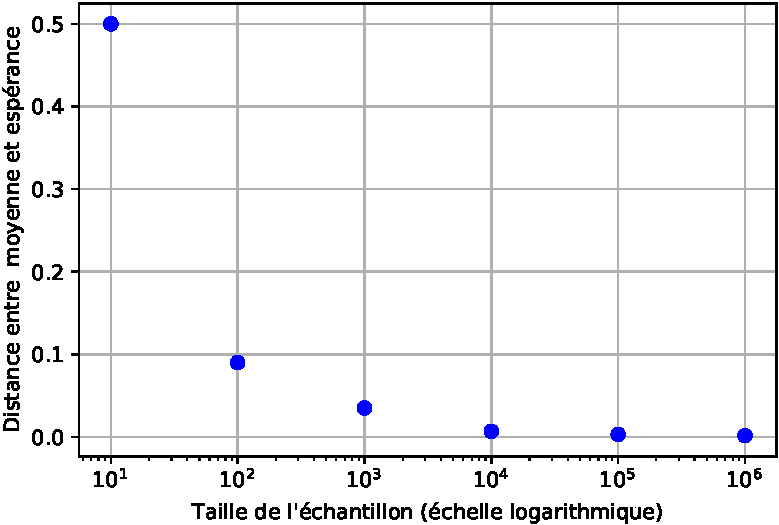
\includegraphics[scale=0.5]{images/distance-moyenne-esperance-crop.pdf}
\end{center}

\end{frame}

\begin{frame}[fragile]
\frametitle{Algorithmique 5,  partie 1}

\texttt{frequence\_fluctuation(va, mu, sigma, N, n)} retourne la fréquence, sur $N$ échantillons de taille $n$ , d'échantillons pour lesquels la moyenne de la variable aléatoire \texttt{va} appartient à  l'intervalle $\Interff{\mu - \frac{\sigma}{2 \sqrt{n}}}{\mu + \frac{\sigma}{2 \sqrt{n}}}$ où $\mu$ et $\sigma$ sont l'espérance et l'écart-type, supposés connus, de la variable aléatoire. 


\begin{lstlisting}[style=rond]
from math import sqrt
from random import random

def frequence_fluctuation(va, mu, sigma, N, n):
    dedans = 0
    rayon = 2 * sigma / sqrt(n)
    for k in range(N):
        if mu - rayon <= moyenne_echantillon(va, n) <= mu + rayon:
            dedans = dedans + 1
    return dedans / n
\end{lstlisting}

\end{frame}


\begin{frame}[fragile]
\frametitle{Algorithmique 5,  partie 2}


On peut observer que la valeur moyenne de la variable aléatoire définie dans \textbf{Algorithme 3} tend presque sûrement vers son espérance  $2$ lorsque la taille de l'échantillon augmente  car la probabilité que $m$ appartienne à l'intervalle $\Interff{\mu - \frac{\sigma}{2 \sqrt{n}}}{\mu + \frac{\sigma}{2 \sqrt{n}}}$ tend vers $0,95$.


\begin{minipage}{0.45\linewidth}
\begin{center}
\fbox{\textbf{Algorithmique 3 \: $N=100$}}

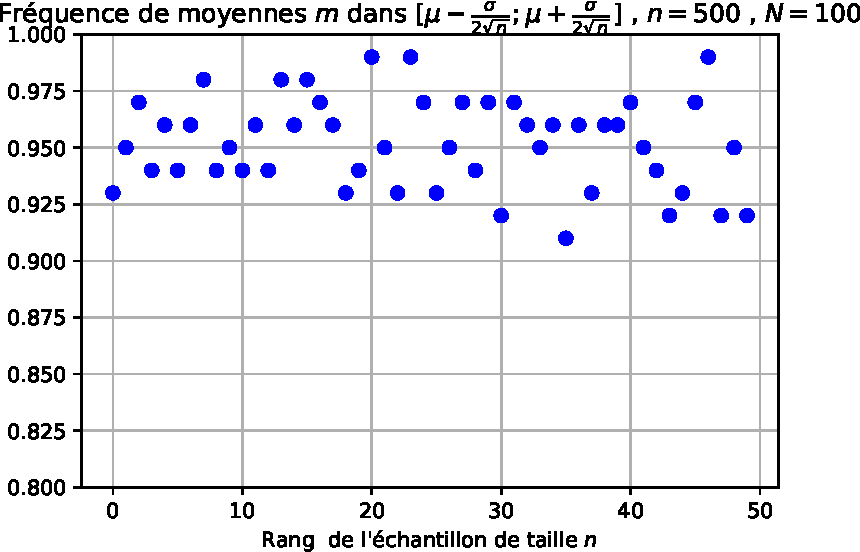
\includegraphics[scale=0.3]{images/frequence-fluctuation-N-100-crop.pdf}
\end{center}
\end{minipage}
\hfill 
\begin{minipage}{0.45\linewidth}
\begin{center}
\fbox{\textbf{Algorithmique 3 \: $N=1000$}}

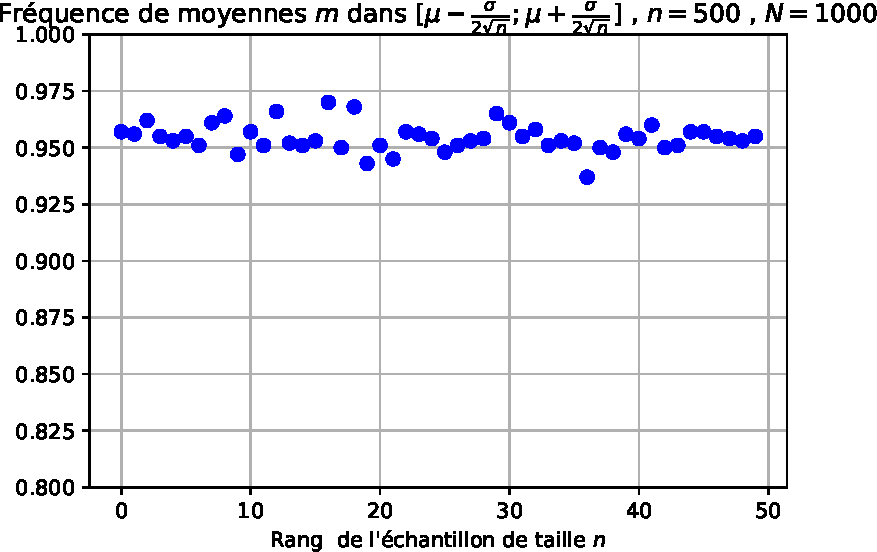
\includegraphics[scale=0.3]{images/frequence-fluctuation-N-1000-crop.pdf}
\end{center}
\end{minipage}



\end{frame}



\begin{frame}[fragile]
\frametitle{Algorithmique 5,  partie 2}



On peut observer que la valeur moyenne de la variable aléatoire définie dans \textbf{Activité 2} tend presque sûrement vers son espérance  $-0,15$ lorsque la taille de l'échantillon augmente car la probabilité que $m$ appartienne à l'intervalle $\Interff{\mu - \frac{\sigma}{2 \sqrt{n}}}{\mu + \frac{\sigma}{2 \sqrt{n}}}$ tend vers $0,95$.


\begin{minipage}{0.45\linewidth}
\begin{center}
\fbox{\textbf{Activité 2 \: $N=100$ } }

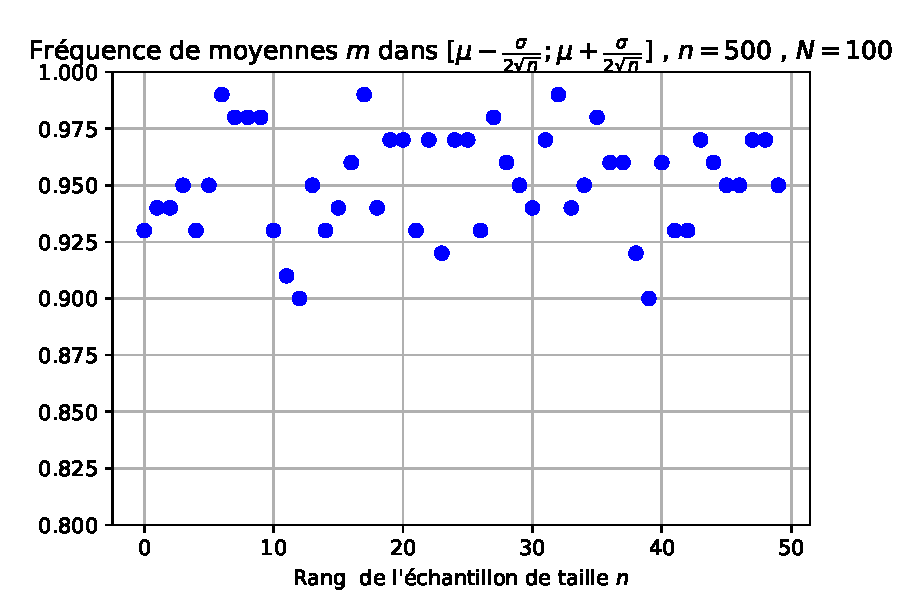
\includegraphics[scale=0.3]{images/frequence-fluctuation-activ2-N-100.pdf}
\end{center}
\end{minipage}
\hfill
\begin{minipage}{0.45\linewidth}
\begin{center}
\fbox{\textbf{Activité 2 \: $N=1000$}}

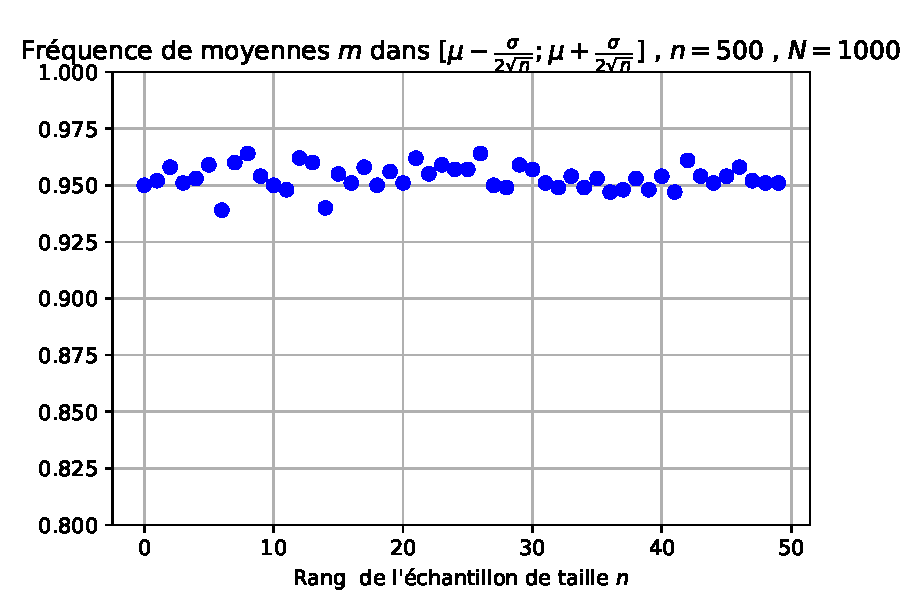
\includegraphics[scale=0.3]{images/frequence-fluctuation-activ2-N-1000.pdf}
\end{center}
\end{minipage}


\end{frame}

\end{document}